Tutti i risultati riportati in questo capitolo sono stati ottenuti sui 109 soggetti del dataset, con la validazione Leave-One-Run-Out descritta nel capitolo precedente e con l’estrazione di feature riemanniana a banco di filtri.

Prima di leggere qualunque cifra occorre fissare due riferimenti. Il primo è il livello del caso, che per una classificazione binaria vale il 50\%. Il secondo è la soglia di significatività: disponendo di circa quarantadue trial indipendenti per soggetto, un classificatore privo di qualunque informazione supera il 50\% piuttosto spesso per effetto del solo caso, e il valore oltre il quale si può escludere questa eventualità con una confidenza del 95\% è pari al \textbf{62,7\%}. Un soggetto che ottenga il 58\% non è un soggetto che funziona male: è un soggetto per il quale non è possibile affermare che abbia prodotto alcun segnale utilizzabile.

\section{Le classificazioni binarie}
Sono state condotte tre distinte classificazioni binarie, tutte sulle run di immaginazione motoria. La prima distingue lo stato di riposo da quello di attivazione, senza interrogarsi su quale movimento venga immaginato; la seconda distingue i pugni dai piedi; la terza il pugno sinistro dal destro.

\begin{table}[htbp]
\centering
\begin{tabular}{lccccc}
\toprule
compito & accuratezza & mediana & dev. std. & scarti & sopra 62,7\% \\
\midrule
riposo / attivazione & 73,61\% & 73,01\% & 10,60 & 25,8\% & 90/109 \\
pugni / piedi        & 69,98\% & 71,67\% & 16,02 & 19,1\% & 69/109 \\
sinistra / destra    & 62,55\% & 59,03\% & 14,69 & 22,1\% & 48/109 \\
\bottomrule
\end{tabular}
\caption{Prestazione media sui 109 soggetti nelle tre classificazioni binarie. L’accuratezza è la balanced accuracy calcolata sulle sole finestre accettate, e va letta congiuntamente alla percentuale di finestre scartate riportata nella penultima colonna.}
\label{tab:binarie}
\end{table}

\begin{figure}[htbp]
\centering
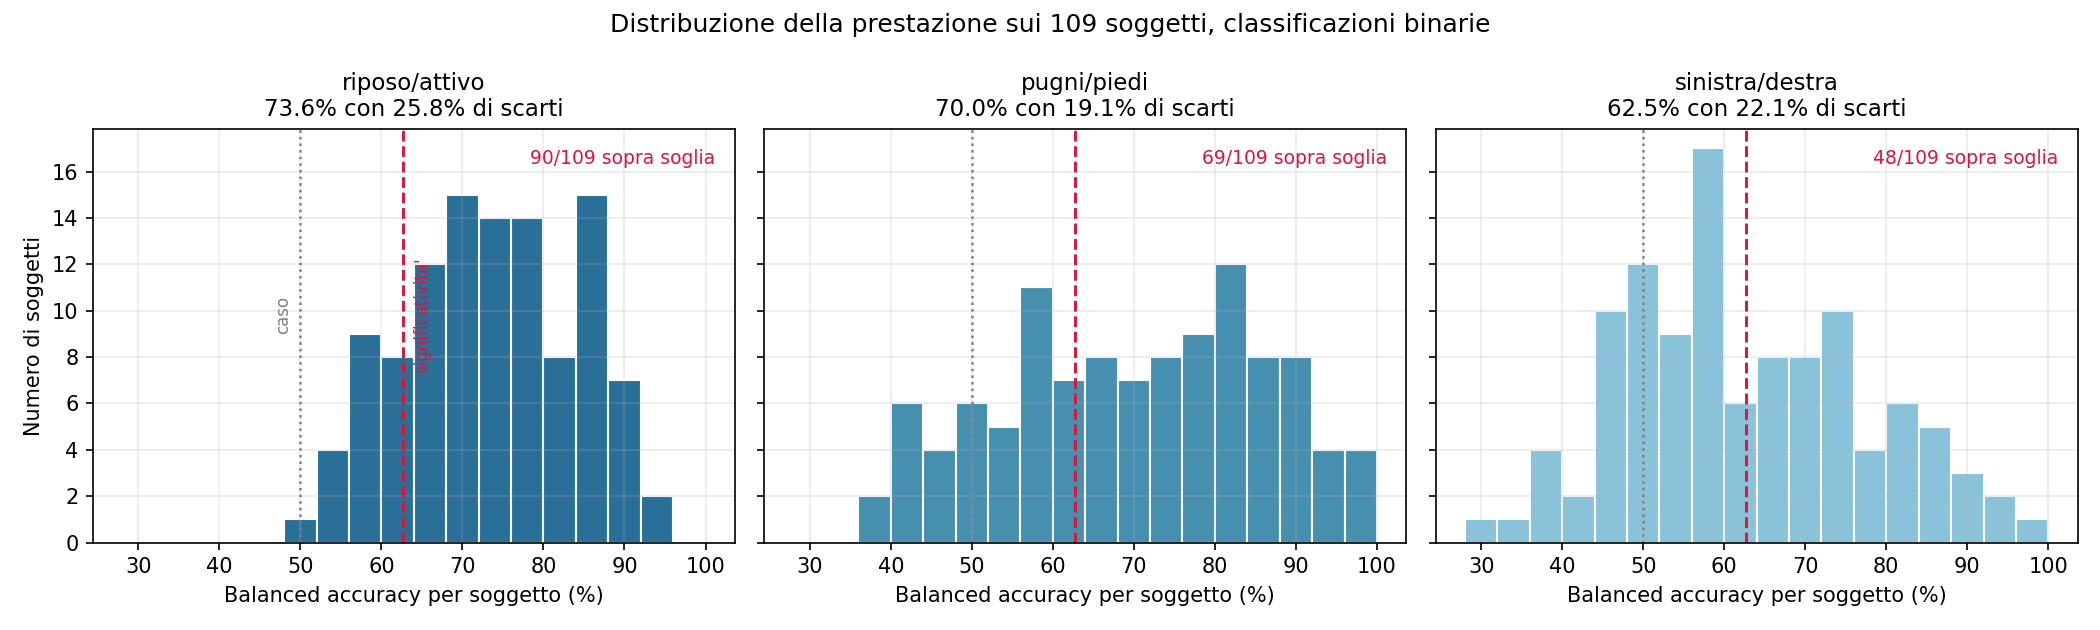
\includegraphics[width=\textwidth]{figure/Grafici/risultati_binari.png}
\caption{Distribuzione della prestazione individuale nei tre compiti. La linea punteggiata indica il livello del caso, quella tratteggiata la soglia di significatività.}
\label{fig:binarie}
\end{figure}

L’ordinamento dei tre compiti corrisponde a quanto ci si attende sul piano neurofisiologico. Riconoscere se il soggetto stia immaginando qualcosa è il compito più semplice, perché la desincronizzazione interessa entrambi gli emisferi e il contrasto da rilevare è una differenza di livello complessivo. Più difficile è la classificazione dei pugni rispetto ai piedi, ma i risultati rimangono buoni poiché le due aree corticali coinvolte, laterale l’una e mediale l’altra, sono ben separate nello spazio. Distinguere la mano sinistra dalla destra, infine, è il compito più arduo, perché le due aree sono simmetriche e vicine e il contrasto è una sottile asimmetria fra emisferi.

La figura \ref{fig:binarie} mostra però che la media riassume assai poco. In tutti e tre i compiti la distribuzione è ampia e attraversa la soglia di significatività: nel caso sinistra contro destra la deviazione standard è di quasi quindici punti e i soggetti vanno dal 29,97 al 97,07\%. Soltanto 48 soggetti su 109, ossia il 44\%, superano la soglia di significatività nella classificazione sinistra contro destra; sono 69 per pugni contro piedi e 90 per riposo contro attivazione.

\subsection{Il ruolo dei campioni scartati}
La colonna degli scarti della tabella \ref{tab:binarie} indica un parametro fondamentale per la corretta lettura dei risultati dei modelli riportati.

Utilizzando un approccio probabilistico, tramite la chiamata al metodo \texttt{grid.\allowbreak predict\_proba(X\_test)}, si è sviluppato un meccanismo di selezione delle finestre che fa sopravvivere solo quelle a cui il modello associa una maggiore certezza: ogni classificazione del modello viene scartata se il grado di certezza ad essa associato non supera una determinata soglia. 

Il numero di finestre (o, ugualmente, di classificazioni) scartate varia da soggetto a soggetto attraverso i tre parametri \texttt{START\_THRESHOLD(0.90)}, \texttt{MIN\_THRESHOLD(0.50)} e \texttt{MIN\_ACCEPTED\_RATIO(0.70)}: la soglia iniziale è pari a 0,90 e a questa il modello sottrae una quantità fissa pari a 0,05 fino a che non viene accettato almeno il 70\% delle classificazioni o fino al raggiungimento della soglia minima. 

Ne consegue che la lettura dell'accuratezza deve essere effettuata congiuntamente al relativo valore di finestre scartate. È possibile apprezzare tale fattore nei risultati della tabella \ref{tab:binarie}: la differenza di accuratezza media tra i compiti della prima e della seconda riga, pari a circa 4 punti percentuali, è sensibilmente assottigliata dalla differenza della percentuale delle finestre scartate, pari a 6,7 punti percentuali.

L'impiego di questa metodologia deriva da osservazioni di natura tecnica: in un sistema BCI reale e online l'omissione di un comando costituisce un disagio modesto, mentre l'accettazione di una classificazione errata risulta più fastidiosa per l'utente finale.

\subsection{Il confronto con e senza scarto}
Per quantificare il contributo della soglia probabilistica, la classificazione pugni contro piedi è stata ripetuta con la medesima pipeline ma con soglia nulla, accettando dunque tutte le finestre. A livello di popolazione il guadagno appare modesto: l'accuratezza media passa dal 67,53 al 69,98\%, ossia \textbf{meno di due punti e mezzo} a fronte del 19,1\% di finestre scartate.

La media, tuttavia, mescola soggetti per i quali lo scarto ha effetti molto diversi. Nella tabella \ref{tab:scarto} i soggetti sono suddivisi in quartili secondo l'accuratezza ottenuta senza scarto, così che il raggruppamento non dipenda dalla grandezza che si vuole confrontare.

\begin{table}[htbp]
\centering
\begin{tabular}{lcccc}
\toprule
quartile & senza scarto & con scarto & guadagno & scarti \\
\midrule
primo (78--98\%)   & 87,04\% & 89,43\% & +2,40 &  8,4\% \\
secondo (68--78\%) & 73,40\% & 77,90\% & +4,51 & 20,1\% \\
terzo (56--68\%)   & 61,57\% & 64,24\% & +2,67 & 23,6\% \\
quarto (38--55\%)  & 48,81\% & 49,13\% & +0,32 & 24,1\% \\
\bottomrule
\end{tabular}
\caption{Classificazione pugni/piedi con e senza scarto delle finestre, per quartili di soggetti ordinati secondo l'accuratezza senza scarto.}
\label{tab:scarto}
\end{table}

Il quadro che ne emerge è diverso da quello suggerito dalla media. Per i soggetti del primo quartile lo scarto riduce l'errore dal 13,0 al 10,5\%, quasi un quinto degli errori in meno, rinunciando però soltanto all'8,4\% delle finestre; per i dieci soggetti migliori gli scarti scendono al 3,9\%. All'estremo opposto, nel quarto quartile viene scartata una finestra su quattro senza alcun beneficio apprezzabile: quando il classificatore non dispone di informazione utile, anche le sue predizioni più sicure sono casuali, e la soglia si limita a ridurre il numero di comandi emessi.

Il basso guadagno medio non indica dunque che la soglia sia inefficace, bensì che la gran parte degli scarti si concentra sui soggetti per i quali non vi è nulla da recuperare. Per i soggetti che producono un segnale utilizzabile, lo scarto rimuove proprio le finestre ambigue a un costo contenuto, confermando ancora una volta che l'effetto di una scelta di progetto dipende in primo luogo dalla persona.


\section{La coerenza della prestazione fra compiti}
Il dato più rilevante della sezione precedente non è la prestazione media del metodo, bensì l’ampiezza della dispersione fra soggetti. Si pone allora la domanda se tale dispersione rifletta una proprietà stabile della persona oppure sia il risultato di fluttuazioni casuali.

\begin{figure}[htbp]
\centering
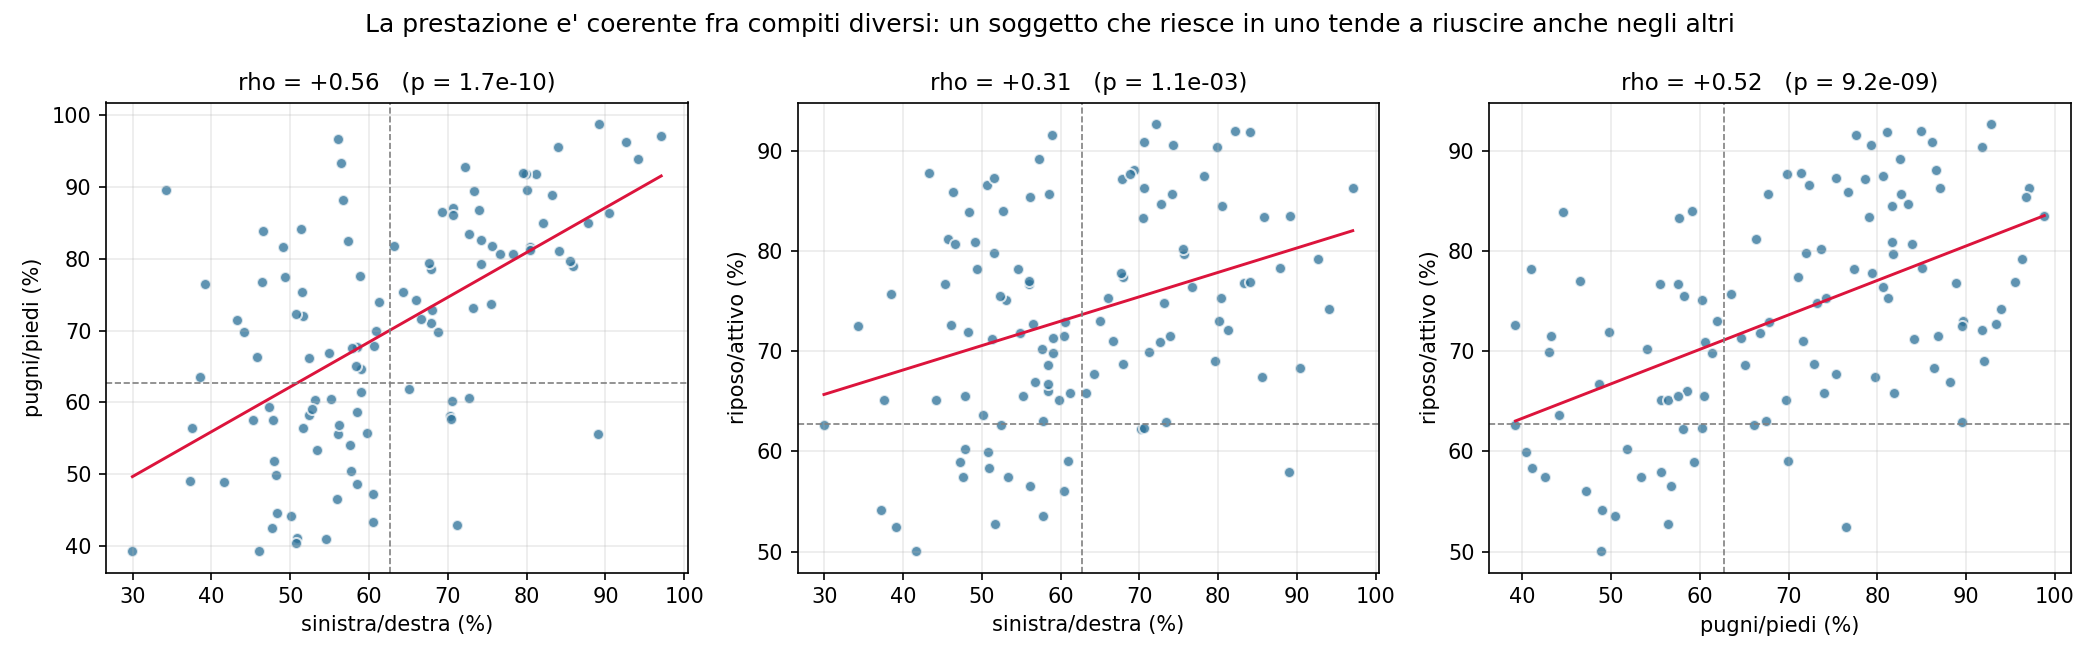
\includegraphics[width=\textwidth]{figure/Grafici/coerenza_soggetti.png}
\caption{Prestazione dei medesimi soggetti in coppie di compiti differenti. Ogni punto rappresenta un soggetto.}
\label{fig:coerenza}
\end{figure}

La risposta, riportata in figura \ref{fig:coerenza}, è netta. Le prestazioni dei medesimi soggetti in compiti diversi sono correlate in misura considerevole: il coefficiente di Spearman vale 0,564 fra sinistra/destra e pugni/piedi, 0,516 fra pugni/piedi e riposo/attivazione e 0,308 fra sinistra/destra e riposo/attivazione. Un soggetto che riesce in un compito tende a riuscire anche negli altri, che sono classificazioni distinte, addestrate separatamente e condotte su registrazioni differenti.

La conclusione è che la variabilità osservata non è rumore ma \textbf{riflette caratteristiche stabili del soggetto}, almeno all'interno della singola sessione di registrazione: l'impiego di metodi differenti (di cui, si ricorda, è stato riportato esclusivamente l'ultimo modello) e le classificazioni binarie di diversa natura confermano la validità delle singole strategie ed evidenziano la possibilità di estrarre dati utili anche con un ridotto numero di campioni.

\section{Il sistema completo a cascata}
I risultati finora mostrati sono stati sufficientemente incoraggianti per sviluppare un \textbf{sistema completo a cascata}, caratterizzato da due stadi distinti di classificazione. Il primo stadio stabilisce se la finestra corrente appartiene alla classe di attivazione oppure no e, in caso di esito positivo, delega al secondo stadio la scelta della precisa classe di attivazione.
Il sistema a due stadi è stato valutato sull’unione di due run tenute fuori contemporaneamente, una per ciascuna famiglia di compiti, così da disporre nell’insieme di test di tutte e cinque le classi finali: riposo, pugno sinistro, pugno destro, entrambi i pugni ed entrambi i piedi. Il livello del caso è dunque il 20\%.

\begin{figure}[htbp]
\centering
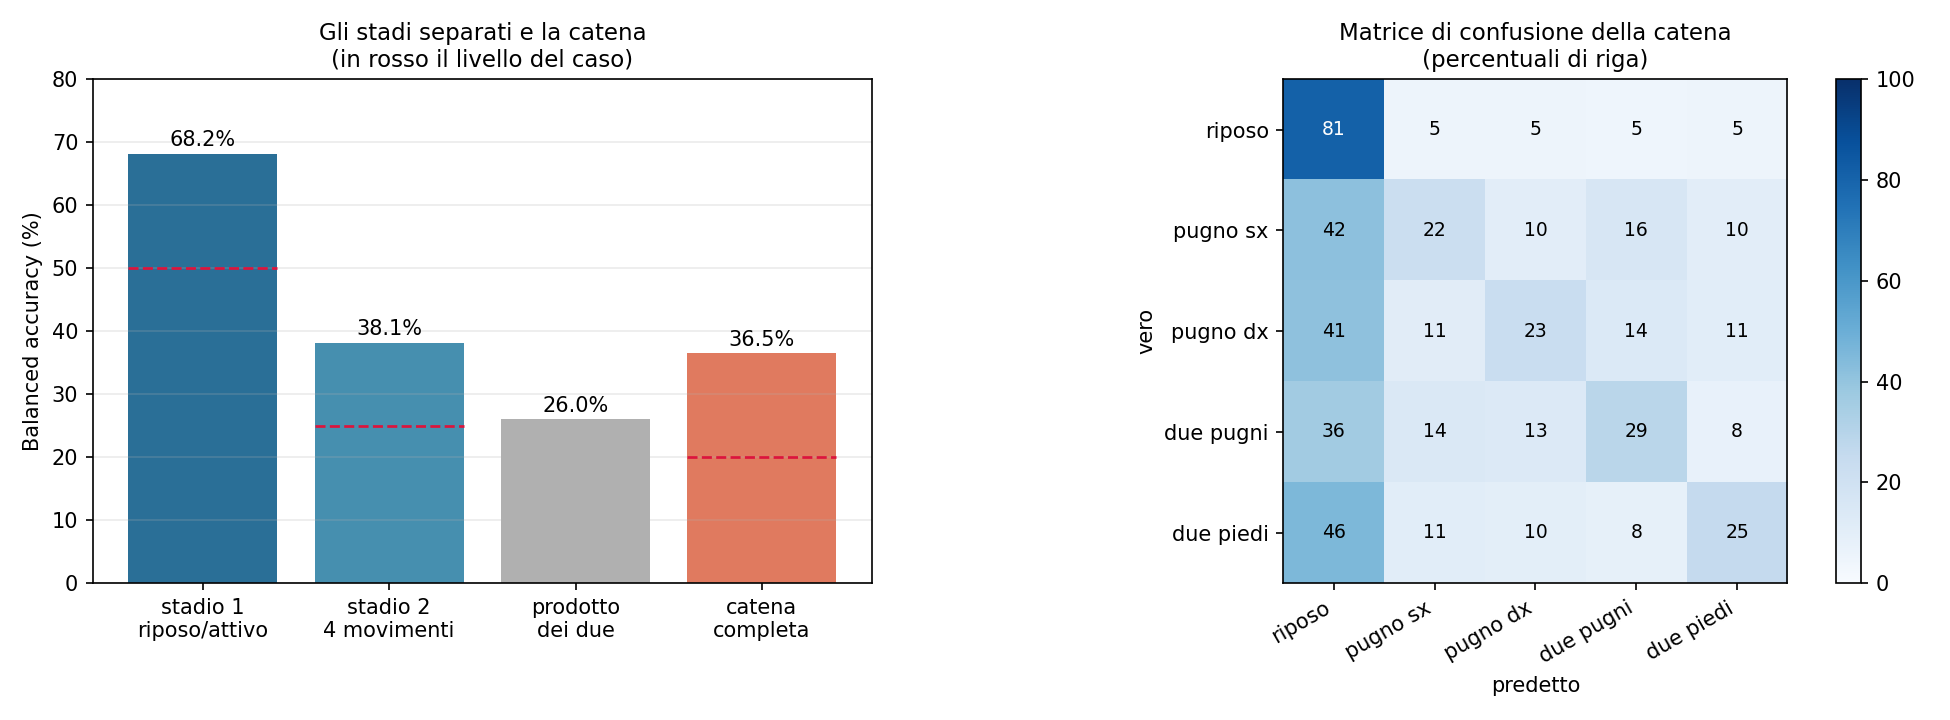
\includegraphics[width=\textwidth]{figure/Grafici/cascata.png}
\caption{A sinistra le prestazioni dei due stadi valutati separatamente, il loro prodotto, da intendersi come riferimento indicativo, e la catena effettiva; in rosso il livello del caso di ciascuno. A destra la matrice di confusione della catena, normalizzata per riga.}
\label{fig:cascata}
\end{figure}

Il primo stadio raggiunge il 68,18\% e il secondo il 38,13\% su quattro classi, quest’ultimo valutato sulle finestre effettivamente attive, ossia supponendo che il primo stadio non commetta errori. La catena completa consegue il 36,46\% con il 26,3\% di campioni scartati.

Come termine di confronto per la catena si può utilizzare il prodotto delle accuratezze dei due stadi, pari al 25,99\%, che rappresenta in modo semplice l'accumularsi degli errori lungo i due livelli. Si tratta però di un riferimento puramente indicativo: il prodotto presuppone che gli errori dei due stadi siano indipendenti, mentre è ragionevole attendersi che le finestre difficili per il primo stadio lo siano anche per il secondo; inoltre la classe di riposo attraversa il solo primo stadio, e la catena è valutata sulle sole finestre accettate. Con queste cautele, la catena consegue il 36,46\%, un valore superiore al riferimento, risultato al quale contribuisce anche la composizione morbida delle probabilità: uno stadio sicuro compensa un secondo stadio tiepido, e i casi nei quali nessuno dei due risulta convinto vengono scartati anziché trasformarsi in errori. Il difetto classico delle architetture in cascata, per cui un errore commesso al primo livello non è più recuperabile, viene in tal modo attenuato.

La matrice di confusione di figura \ref{fig:cascata} indica però con chiarezza dove il sistema perda. La classe di riposo viene riconosciuta nel 78\% dei casi, mentre ciascuna classe di movimento viene ricondotta al riposo in una percentuale compresa fra il 25 e il 35\%. Il collo di bottiglia non è dunque la discriminazione fra i quattro movimenti bensì la \textbf{sensibilità del primo stadio}, che lascia sfuggire una quota consistente delle attivazioni: un movimento non rilevato al primo livello è definitivamente perduto.

\section{Le prestazioni migliori}
Le medie riportate finora descrivono la popolazione nel suo insieme, ma dicono poco su quanto l'algoritmo sia in grado di ottenere quando il soggetto produce un segnale utilizzabile. Per rispondere a questa domanda la tabella \ref{tab:migliori} riporta, per ciascun compito, il soggetto migliore e la media del 10\% migliore della popolazione, ossia gli undici soggetti con l'accuratezza più elevata. Il secondo dato è il più significativo, perché meno esposto alla fortuna di un singolo soggetto.

\begin{table}[htbp]
\centering
\begin{tabular}{lccccc}
\toprule
compito & \multicolumn{2}{c}{soggetto migliore} & \multicolumn{2}{c}{10\% migliore} & sopra 90\% \\
 & accuratezza & scarti & accuratezza & scarti & \\
\midrule
riposo / attivazione & 92,69\% & 24,5\% & 90,26\% & 24,2\% & 7/109 \\
pugni / piedi        & 98,80\% &  0,4\% & 94,56\% &  4,2\% & 11/109 \\
sinistra / destra    & 97,07\% &  4,8\% & 89,05\% & 11,7\% & 4/109 \\
cascata (5 classi)   & 75,54\% & 28,3\% & 61,72\% & 27,2\% & 0/109 \\
\bottomrule
\end{tabular}
\caption{Prestazione del soggetto migliore e media degli undici soggetti migliori per ciascun compito. Per la cascata il livello del caso è il 20\%.}
\label{tab:migliori}
\end{table}

Il quadro è molto diverso da quello delle medie. Nella classificazione pugni contro piedi gli undici soggetti migliori superano in media il 94\% scartando appena il 4\% delle finestre, e il migliore sbaglia poco più di una finestra su cento. Anche nel compito sinistra contro destra, il più arduo e quello con la media più bassa, il 10\% migliore si attesta intorno all'89\%. Nel sistema a cascata, dove il caso vale il 20\%, il soggetto migliore riconosce correttamente tre finestre su quattro fra cinque classi.

Due osservazioni impediscono di attribuire questi valori al caso. La prima è che si collocano ben oltre la soglia di significatività del 62,7\%: il massimo su 109 soggetti è per costruzione un dato ottimistico, ma nessuna fluttuazione casuale su circa quarantadue trial può portare un classificatore privo di informazione oltre il 90\%. La seconda è che \textbf{i soggetti migliori sono sempre gli stessi}: i soggetti 029, 042 e 062 compaiono fra i cinque migliori sia nel compito pugni/piedi sia in quello sinistra/destra sia nella cascata, coerentemente con quanto osservato nella sezione sulla coerenza fra compiti.

Questi risultati vanno letti alla luce delle condizioni descritte nell'introduzione. I soggetti non avevano ricevuto alcun addestramento all'immaginazione motoria, non hanno mai ricevuto un riscontro della propria attività e ciascun modello binario è stato addestrato su appena due run, circa quattro minuti di registrazione. Ciò nonostante, per una parte della popolazione l'algoritmo raggiunge accuratezze paragonabili a quelle di un sistema utilizzabile nella pratica. Il risultato conferma che, \textbf{quando il soggetto produce un ritmo sensomotorio marcato, la pipeline è già in grado di classificarlo con buona accuratezza anche in assenza di qualunque addestramento}, e che la bassa media della popolazione dipende in larga parte dai soggetti che tale segnale non producono.

\section{Il predittore di illiteracy}
Il predittore è stato calcolato su tutti e 109 i soggetti a partire dalla sola run di linea di base, e confrontato con la prestazione conseguita nelle run di compito. Trattandosi di due insiemi di registrazioni disgiunti, fra le due misure non sussiste alcuna forma di circolarità. Anche in questo caso si è fatto uso del coefficiente di Spearman, valutato sulla base del confronto tra il picco dei ritmi mu rispetto al fondo 1/f e l'accuratezza del relativo soggetto.

\begin{table}[htbp]
\centering
\begin{tabular}{lcc}
\toprule
configurazione & $\rho$ media dei canali & $\rho$ minimo fra i canali \\
\midrule
sinistra / destra, canali C3 e C4      & 0,376 & 0,416 \\
pugni / piedi, canali C3, C4 e Cz      & 0,443 & 0,372 \\
\bottomrule
\end{tabular}
\caption{Correlazione di Spearman fra la prominenza del ritmo sensomotorio a riposo e la prestazione conseguita, su 109 soggetti. Tutti i valori riportati hanno un p-value inferiore a $10^{-3}$.}
\label{tab:predittore}
\end{table}

\begin{figure}[htbp]
\centering
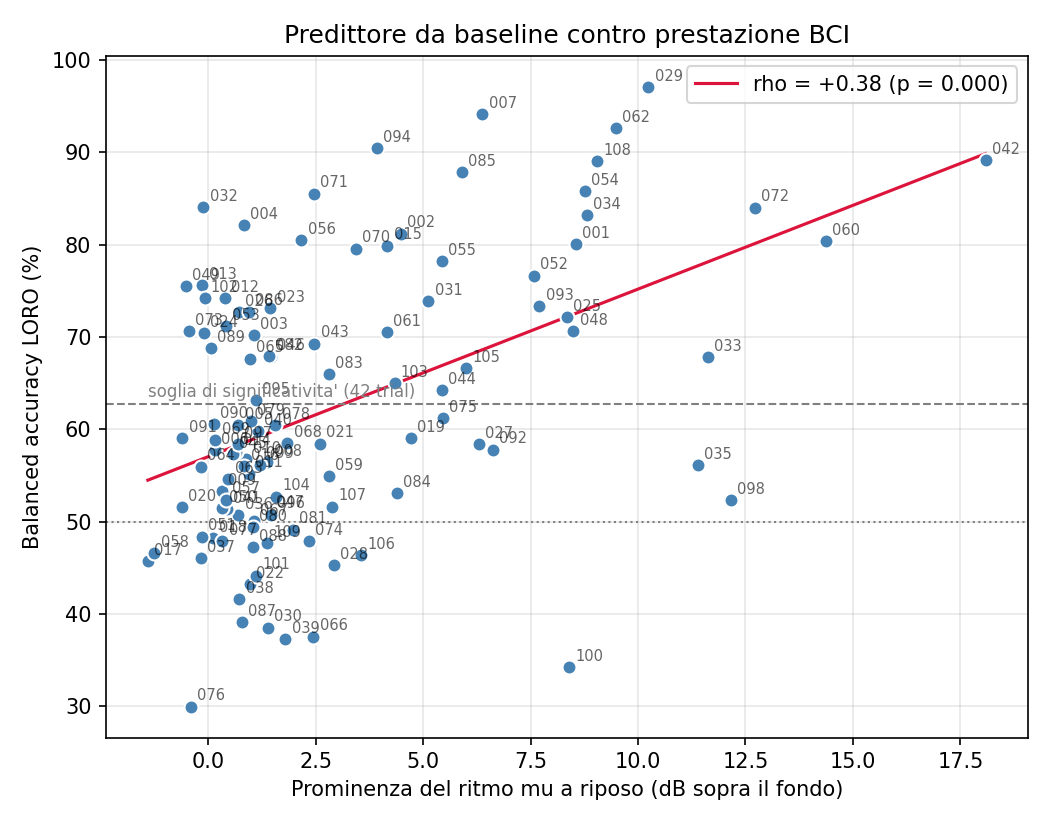
\includegraphics[width=0.49\textwidth]{figure/Grafici/smr_vs_performance.png}
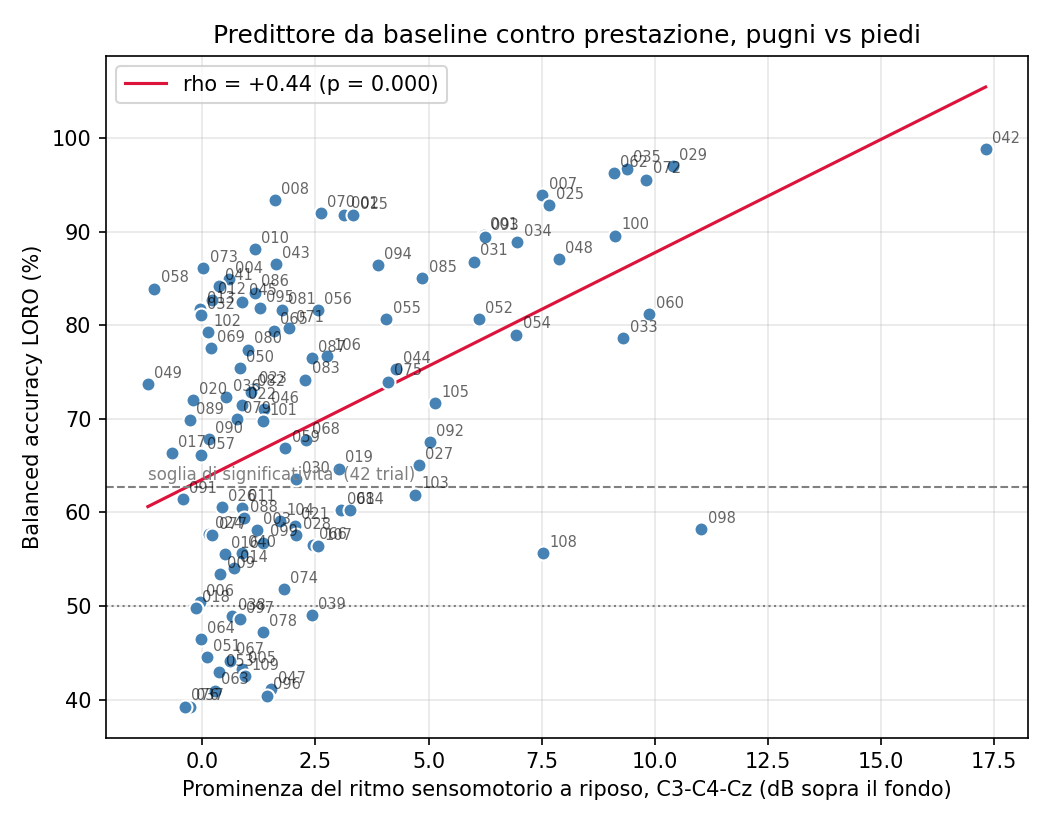
\includegraphics[width=0.49\textwidth]{figure/Grafici/smr_vs_performance_mani_piedi.png}
\caption{Prominenza del ritmo sensomotorio a riposo contro prestazione conseguita: a sinistra per il compito sinistra/destra, a destra per il compito pugni/piedi. Ogni punto è un soggetto.}
\label{fig:predittore}
\end{figure}

Le quattro configurazioni riportate in tabella \ref{tab:predittore} producono coefficienti compresi fra 0,37 e 0,44, nonostante si riferiscano a compiti differenti, a insiemi di elettrodi differenti e a due diverse modalità di aggregazione fra i canali. Un minuto di registrazione a riposo predice la prestazione nella discriminazione fra le due mani press’a poco con la stessa efficacia con cui predice quella fra pugni e piedi.

L’osservazione ha una conseguenza interpretativa precisa. Se il predittore misurasse una capacità specifica del compito, per esempio l’attitudine a lateralizzare l’attività fra i due emisferi, ci si attenderebbe una correlazione sensibilmente più elevata con il compito sinistra contro destra rispetto a quello pugni contro piedi. Il fatto che le due siano quasi equivalenti indica che ciò che viene misurato è \textbf{una proprietà generale del soggetto}, ossia quanto marcata sia la sua attività ritmica sensomotoria, e non la sua abilità in un compito particolare. Il dato è coerente con quanto osservato nella sezione sulla coerenza fra compiti, ed è esattamente ciò che rende il predittore utilizzabile come strumento di selezione preliminare, in quanto indipendente dall’applicazione che si intenda poi realizzare.


\subsection{L’impiego come regola di selezione}
La correlazione misura l’esistenza di una relazione, non la sua utilità pratica. Per valutare quest’ultima si è verificato come vari l’accuratezza media della popolazione al variare della quota di soggetti esclusi sulla base del predittore.

\begin{table}[htbp]
\centering
\begin{tabular}{lcc}
\toprule
soglia sul predittore & soggetti esclusi & accuratezza media dei rimanenti \\
\midrule
nessuna              & 0/109  & 62,55\% \\
10\textsuperscript{o} percentile & 11/109 & 63,39\% \\
20\textsuperscript{o} percentile & 22/109 & 63,64\% \\
30\textsuperscript{o} percentile & 33/109 & 64,16\% \\
40\textsuperscript{o} percentile & 44/109 & 65,44\% \\
\bottomrule
\end{tabular}
\caption{Accuratezza media nel compito sinistra/destra al variare della quota di soggetti esclusi in base al predittore.}
\label{tab:screening}
\end{table}

L’esito, riportato in tabella \ref{tab:screening}, è modesto: escludendo il 40\% della popolazione l’accuratezza media dei rimanenti cresce di meno di tre punti. Con un coefficiente di correlazione di poco superiore a 0,4, del resto, un simile risultato è quello che ci si deve attendere, giacché il predittore spiega una frazione limitata della variabilità osservata.

Occorre inoltre osservare che una tabella di questa natura tende per costruzione a mostrarsi favorevole: escludendo i soggetti peggiori secondo una qualunque grandezza anche debolmente correlata con la prestazione, la media dei rimanenti non può che salire.

\section{Sintesi}
I risultati esposti in questo capitolo possono essere ricondotti a un numero ristretto di osservazioni, che conviene richiamare prima di trarne una conclusione.

Per quanto riguarda i compiti, l'ordinamento delle tre classificazioni binarie rispecchia la difficoltà attesa sul piano neurofisiologico: riposo contro attivazione raggiunge in media il 73,61\%, pugni contro piedi il 69,98 e sinistra contro destra il 62,55, con quote di finestre scartate comprese fra il 19 e il 26\%. Le medie, tuttavia, descrivono male la popolazione: la soglia di significatività del 62,7\% viene superata da 90 soggetti su 109 nel primo compito, da 69 nel secondo e da appena 48 nel terzo, e nel compito sinistra/destra le prestazioni individuali si distribuiscono su un intervallo di quasi settanta punti.

Per quanto riguarda le scelte di progetto, la soglia probabilistica produce in media un guadagno contenuto, inferiore a due punti e mezzo, ma il dato medio nasconde due comportamenti opposti: per i soggetti del primo quartile lo scarto elimina quasi un quinto degli errori rinunciando a meno di una finestra su dieci, mentre per quelli dell'ultimo quartile scarta una finestra su quattro senza alcun beneficio. Il sistema a cascata, pur fermandosi al 36,46\% su cinque classi, si colloca al di sopra del prodotto delle accuratezze dei due stadi, preso come riferimento indicativo, anche grazie alla composizione morbida delle probabilità; il suo limite principale risiede nella sensibilità del primo stadio, che riconduce al riposo fra un quarto e un terzo delle attivazioni.

Per quanto riguarda i soggetti, tre osservazioni distinte puntano nella stessa direzione. La prestazione di un soggetto in un compito è correlata con quella negli altri, con coefficienti di Spearman compresi fra 0,31 e 0,56. I soggetti migliori sono sempre gli stessi e il 10\% superiore della popolazione raggiunge in media il 94,56\% nel compito pugni/piedi e l'89,05 in quello sinistra/destra, pur in assenza di qualunque addestramento. Un solo minuto di registrazione a riposo, infine, predice in parte la prestazione, con coefficienti compresi fra 0,37 e 0,44 che non dipendono in modo apprezzabile dal compito. Quest'ultimo risultato si traduce però in una regola di selezione di efficacia modesta: escludendo il 40\% dei soggetti l'accuratezza media dei rimanenti cresce di meno di tre punti.